\documentclass{article}
\usepackage{tikz, comment}
\usepackage{pifont}
\usepackage{fontspec}
\usetikzlibrary{arrows, decorations.markings, decorations.pathreplacing}
\begin{comment}
:Title: Not defined yet
:Tags: eccentricity of a conic section;focus of a parabola;end behavior;area using polar coordinates, polar integral formula ;moment
:Prob: 0.5279;0.524;0.5231;0.5214;0.5186
:Slug: No name yet

Description Here.........
\end{comment}
\begin{document}\centering

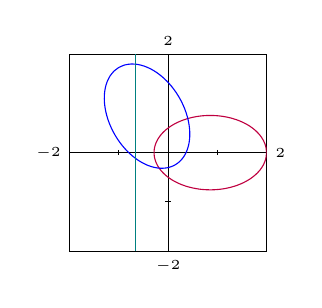
\begin{tikzpicture}[>=latex,xscale=0.25*10/4, yscale=0.25*10/4][font=\sf\small]

%\draw[xstep=0.5cm,ystep=0.5cm,color=gray!20] (-1, -1) (3, 1);

\draw[] (-2, 0) -- (2, 0);
\draw[] (0, -2) -- (0, 2);

\node[left] at (-2, 0) {\tiny$-2$};
\node[right] at (2, 0) {\tiny$2$};
\node[below] at (0, -2) {\tiny$-2$};
\node[above] at (0, 2) {\tiny$2$};

\clip[draw] (-2, -2) rectangle (2, 2);

\draw[purple, samples=100, smooth, domain=0:2*pi, variable=\t]
plot ({2/(4-3*cos(\t r))*cos(\t r)}, {2/(4-3*cos(\t r))*sin(\t r)});

\begin{scope}[rotate around={120:({0}, {0})}]
\draw[blue, samples=100, smooth, domain=0:2*pi, variable=\t]
plot ({2/(4-3*cos(\t r))*cos(\t r)}, {2/(4-3*cos(\t r))*sin(\t r)});

\end{scope}

\draw[teal, samples=100, smooth, domain=-2:2, variable=\y]
plot ({-2/3}, {\y});

\foreach \x in {-1,1}
\draw (\x,2pt/5*4) -- (\x,-2pt/5*4)
node[anchor=north] {}%{\tiny$\x$}
;
\foreach \x in {}
\draw (\x,2pt*2) -- (\x,-2pt*2)
node[anchor=south] {\tiny$\x$}
;
\foreach \y in {-2,-1}
\draw (-2pt/5*4,\y) -- (2pt/5*4,\y)
node[anchor=east] {}%{\tiny $\y$}
;

\end{tikzpicture}
\end{document}